\chapter{Металлические волноводы}
\section{Прямоугольный волновод}

\begin{gather*}
	E_x = \frac{-i}{g^2}\left(h\pder{E_z}{x} + \omega\mu\pder{H_z}{y}\right),\\
	E_y = \frac{-i}{g^2}\left(h\pder{E_z}{y} - \omega\mu\pder{H_z}{x}\right),\\
	H_x = \frac{i}{g^2}\left(\omega\eps\pder{E_z}{y} - h\pder{H_z}{x}\right),\\
	H_y = \frac{-i}{g^2}\left(\omega\eps\pder{E_z}{x} + h\pder{H_z}{y}\right).
\end{gather*}

В системе могут существовать отдельные TE и TM волны, если на контуре волновода
\[
	\pder{E_z}{l} = \pder{H_z}{l} = 0.
\]
Если условие не выполняются, то в системе будут наблюдаться гибридные волны.

Рассмотрим прямоугольный волновод \( a \times b, a > b, a || Ox \).

E-волны (TM) имеют в нём следующий вид:

\begin{align*}
	& E_z = E_0\sin\frac{m\pi x}{a}\sin\frac{n\pi y}{b},\\
	& H_z = 0,\\
	& E_x = -i\frac{hm\pi}{g_{m,n}^2a}E_0\cos\frac{m\pi x}{a}\sin\frac{n\pi y}{b},\\
	& E_y = -i\frac{hn\pi}{g_{m,n}^2b}E_0\sin\frac{m\pi x}{a}\cos\frac{n\pi y}{b},\\
	& H_x = -\frac{\omega\eps}{h}E_y = i\frac{\omega\eps n\pi}{g_{m,n}^2b}E_0
	 								\sin\frac{m\pi x}{a}\cos\frac{n\pi y}{b},\\
	& H_y = \frac{\omega\eps}{h}E_x = -i\frac{\omega\eps m\pi}{g_{m,n}^2a}E_0
	 								\cos\frac{m\pi x}{a}\sin\frac{n\pi y}{b}.
\end{align*}

H-волны (TE):
\begin{align*}
	& E_z = 0,\\
	& H_z = H_0\cos\frac{m\pi x}{a}\cos\frac{n\pi y}{b},\\
	& E_x = i\frac{\omega\mu n\pi}{g_{m,n}^2b}H_0\cos\frac{m\pi x}{a}\sin\frac{n\pi y}{b},\\
	& E_y = -i\frac{\omega\mu m\pi}{g_{m,n}^2a}H_0\sin\frac{m\pi x}{a}\cos\frac{n\pi y}{b},\\
	& H_x = -\frac{h}{\omega\mu}E_y = i\frac{hm\pi}{g_{m,n}^2a}H_0
	 								\sin\frac{m\pi x}{a}\cos\frac{n\pi y}{b},\\
	& H_y = \frac{h}{\omega\mu}E_x = -i\frac{h n\pi}{g_{m,n}^2b}H_0
	 								\cos\frac{m\pi x}{a}\sin\frac{n\pi y}{b}.
\end{align*}

Здесь \( g_{m,n} \) -- поперечное волновое число, определяемое выражением
\[
	g_{m,n} = \pi\sqrt{\frac{m^2}{a^2} + \frac{n^2}{b^2}}.
\]

Так как
\[
	h^2 = \beta^2 - g_{m,n}^2,
\]
то для данного типа волны существует критическая частота, ниже которой эта волна возбуждаться не может. Она называется критической:
\[
	\omega_c = \frac{c}{\sqrt{\eps_r \mu_r}}g_{m,n}.
\]

Дисперсионное соотношение имеет вид:
\[
	h^2 = \frac{\omega^2 \eps_r \mu_r}{c^2} - g_{m,n}^2,
\]
откуда
\[
	v_p = \frac{\omega}{h} = \frac{c}{\sqrt{\eps_r\mu_r}}\frac{1}{\sqrt{1 - \omega_c^2 / \omega^2}},
\]

\[
	v_g = \der{\omega}{h} = \frac{c}{\sqrt{\eps_r\mu_r}}\sqrt{1 - \omega_c^2 / \omega^2}.
\]

Заметим, что
\[
	v_p v_g = \frac{c^2}{\eps_r\mu_r} \text{ --- квадрат скорости света в среде.}
\]

\begin{center}
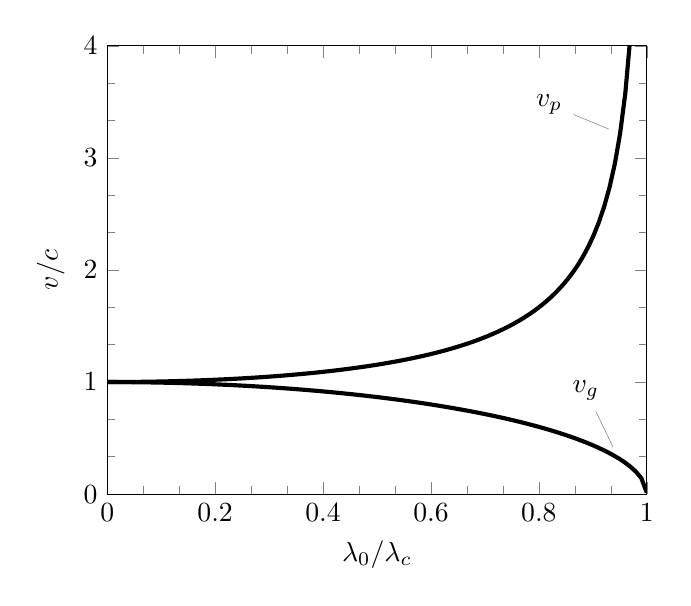
\begin{tikzpicture}
\begin{axis}[
	xmin = 0, xmax = 1, ymin = 0, ymax = 4,
    xlabel = {$\lambda_0 / \lambda_c$},
    ylabel = {$v / c$},
    minor tick num = 2
]
\addplot[domain=0:0.97,samples=100,line width=1.5pt]{(1 - x^2)^-0.5} node[pos=0.75,pin=170:{$v_p$}]{};
\addplot[domain=0:1,samples=100,line width=1.5pt]{sqrt(1 - x^2)} node[pos=0.8,pin=100:{$v_g$}]{};
\end{axis}
\end{tikzpicture}
\end{center}


Относительное расположение критических длин волн:
\begin{center}
	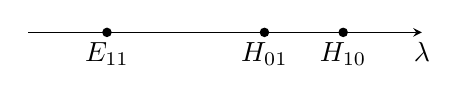
\begin{tikzpicture}[>=stealth]
		\draw[->](0,0) -- (5,0);
		\draw[fill] (1,0) circle(1.5pt) node[below]{$E_{11}$};
		\draw[fill] (3,0) circle(1.5pt) node[below]{$H_{01}$};
		\draw[fill] (4,0) circle(1.5pt) node[below]{$H_{10}$};
		\draw (5,0) node[below]{$\lambda$};
	\end{tikzpicture}
\end{center}

Характеристические сопротивления для волн:
\begin{align*}
	Z_c^E = & \sqrt{\frac{E_xE_x^* + E_yE_y^*}{H_xH_x^* + H_yH_y^*}} = \frac{h}{\omega\eps} = Z_c\sqrt{1 - \frac{\lambda_0^2}{\lambda_c^2}},\\
	Z_c^H = & \sqrt{\frac{E_xE_x^* + E_yE_y^*}{H_xH_x^* + H_yH_y^*}} = \frac{\omega\mu}{h} = \frac{Z_c}{\sqrt{1 - \frac{\lambda_0^2}{\lambda_c^2}}}.
\end{align*}

Рассмотрим передачу мощности в волне \( H_{10} \):
\[
	\Pi_z = -\frac{1}{2}E_y H_x^* = \frac{1}{2}\frac{h}{\omega\mu}E_yE_y^* = \frac{h}{2\omega\mu}\omega^2\mu^2 H_0^2\sin^2\frac{\pi x}{a} = \frac{\omega\mu h}{2}H_0^2\sin^2\frac{\pi x}{a},
\]
\[
	h= \frac{2\pi}{\lambda_0}\sqrt{1 - \frac{\lambda_0^2}{4a^2}},
\]
\[
	\Pi_z = \frac{\mu ca^2}{\pi\lambda_0^2}\sqrt{1 - \frac{\lambda_0^2}{4a^2}}H_0^2\sin^2\frac{\pi x}{a},
\]
а передаваемая мощность определяется интегралом по поперечному сечению:
\[
	P = \frac{\mu ca^3b}{2\pi\lambda_0^2}\sqrt{1 - \frac{\lambda_0^2}{4a^2}}H_0^2 = \frac{abh}{4\omega\mu}E_{max}^2.
\]

\section{Коаксиальный волновод}
\begin{gather*}
	E_r =    \frac{-i}{g^2}\left(h\pder{E_z}{r} + \frac{\omega\mu}{r}\pder{H_z}{\phi}\right),\\
	E_\phi = \frac{-i}{g^2}\left(\frac{h}{r}\pder{E_z}{\phi} - \omega\mu\pder{H_z}{r}\right),\\
	H_r =    \frac{i}{g^2}\left(\frac{\omega\eps}{r}\pder{E_z}{\phi} - h\pder{H_z}{r}\right),\\
	H_\phi = \frac{-i}{g^2}\left(\omega\eps\pder{E_z}{r} + \frac{h}{r}\pder{H_z}{\phi}\right).
\end{gather*}

Основной режим работы -- TEM-волны, волноводные гармоники -- паразитные.

\[
	\Delta_\perp E_z = g^2 E_z = 0,\quad \Delta_\perp H_z = g^2 H_z = 0.
\]
с граничными
\[
	\left.E_\tau\right|_{r=a,b} = 0 \Rightarrow \left.E_z\right|_{r=a,b} = 0, \left.\pder{H_z}{r}\right|_{r=a,b} = 0
\]
\[
	\frac{1}{r}\pder{}{r}\left( rE_z \right) + \frac{1}{r^2}\ppder{E_z}{\phi} + g^2E_z = 0.
\]
\[
	E_z = [AJ_m(gr) + BN_m(gr)]\cos(m\phi)
\]
При \( b = 0 \) \( B = 0 \)
\[
	E_z = E_0J_m(gr)\cos(m\phi).
\]
Поперечные волновые числа определяются из условия
\[
	J_m(ga) = 0,\ g_{mn} = \frac{\nu_{mn}}{a}.
\]

\begin{align*}
	E_z &= E_0 J_m(\frac{\nu_{mn}}{a}r)\Phi(m\phi),\\
	E_r &= -\frac{iha}{\nu_{mn}}E_0 J_m'(\frac{\nu_{mn}}{a}r)\Phi(m\phi),\\
	E_\phi &= -\frac{iha^2m}{\nu_{mn}^2r}E_0 J_m(\frac{\nu_{mn}}{a}r)\Phi'(m\phi),\\
	H_z &= 0,\\
	H_r &= -\frac{\omega\eps}{h}E_\phi,\\
	H_\phi &= \frac{\omega\eps}{h}E_r.
\end{align*}


Рассмотрим теперь \( H \)-волны:
\[
	\Delta_\perp H_z + g^2H_z = 0,\quad \left.\pder{H_z}{n}\right|_{r=a,b}= 0
\]

\[
	H_z = [AJ_m(gr) + BN_m(gr)]\Phi(m\phi)
\]

Если \( b=0 \), то в силу ограниченности поля \(B = 0\), а дисперсионное соотношение имеет вид
\[
	J_m'(ga) = 0 \Rightarrow ga = \mu_{mn}, g_{mn} = \frac{\mu_{mn}}{a}, \lambda_c = \frac{2\pi a}{\mu_{mn}}, \mu_{11} = 1.841.
\]

Поля в волноводе имеют вид:
\begin{align*}
	H_z &= H_0 J_m(\frac{\mu_{mn}}{a}r)\Phi(m\phi),\\
	E_r &= -\frac{i\omega\mu a^2m}{r\mu_{mn}^2}H_0 J_m(\frac{\mu_{mn}}{a}r)\Phi'(m\phi),\\
	E_\phi &= \frac{i\omega\mu a}{\mu_{mn}}E_0 J_m'(\frac{\mu_{mn}}{a}r)\Phi(m\phi),\\
	E_z &= 0,\\
	H_r &= -\frac{h}{\omega\mu}E_\phi,\\
	H_\phi &= \frac{h}{\omega\mu}E_r.
\end{align*}

Для коаксиального волновода имеем
\[
	\begin{cases}
		AJ_m'(gb) + BN_m'(gb) = 0,\\
		AJ_m'(ga) + BN_m'(ga) = 0.\\
	\end{cases},
	\quad
	J_m'(gb)N_m'(ga) - J_m'(ga)N_m'(gb) = 0
\]

Характеристическое сопротивление волновода
\[
	Z_c = \frac{E_\perp}{H_\perp}.
\]
